% 0467(본책 84쪽) — 원, 두 현 AC·BD 의 교점 P, ∠APB 표시. 스캔 삽화를 TikZ 로 다시 그림. 답은 적지 않는다.
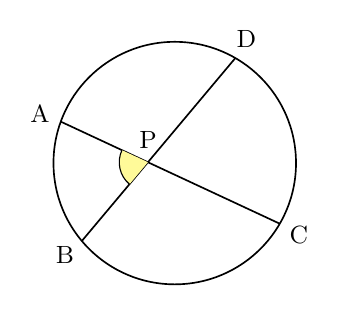
\begin{tikzpicture}[scale=1.4, line width=0.6pt]
  \draw (0.000,0.000) circle (1.100);
  \draw (-1.034,0.376) -- (0.953,-0.550);
  \draw (-0.843,-0.707) -- (0.550,0.953);
  \fill[yellow!40] (-0.243,0.008) -- (-0.479,0.117) arc (155.0:230.0:0.260) -- cycle;
  \draw[line width=0.4pt] (-0.479,0.117) arc (155.0:230.0:0.260);
  \node[font=\small, inner sep=1pt] at (-1.222,0.445) {A};
  \node[font=\small, inner sep=1pt] at (-0.996,-0.836) {B};
  \node[font=\small, inner sep=1pt] at (1.126,-0.650) {C};
  \node[font=\small, inner sep=1pt] at (0.650,1.126) {D};
  \node[font=\small, inner sep=1pt] at (-0.243,0.208) {P};
\end{tikzpicture}
